\documentclass[a4paper]{article}
\usepackage[T1]{fontenc}
\usepackage[utf8]{inputenc}
\usepackage[english]{babel}

\usepackage{amsmath}
\usepackage{amssymb}
\usepackage{a4wide}
\usepackage{dsfont}
\usepackage{lmodern}
\usepackage{listings}
\usepackage{graphicx}
\usepackage{float}
\usepackage[strict]{changepage} % Use to change pagedimensions
\usepackage[font=footnotesize,labelfont=bf]{caption}
\usepackage{subcaption}
\usepackage{bm}

\setlength{\parindent}{0pt}

\title{\textbf{Assignment 2 - resubmission} \\ \small Statistical Methods for Machine Learning }
\author{\textbf{Group members}\\
        Ásbjørn Viderø Jøkladal\\
        Martin Holm Cservenka\\
        Tue Haulund}
\date{10\textsuperscript{th} of March, 2015}

%=======================================================================
\begin{document}
\maketitle
\tableofcontents
\newpage
%=======================================================================

\section{Classification}

\subsection{Linear discriminant analysis}
Upon execution of the implemented linear discriminant analysis of the training- and test-set, the following accuracy results are obtained
\begin{figure}[H]
	\begin{lstlisting}
	Accuracy of LDA on training dataset: 0.86
	Accuracy of LDA on test dataset: 0.815789473684
	\end{lstlisting}
	\caption{Training and test accuracy results of the implemented LDA algorithm}
	\label{fig:lda_results}
\end{figure}

\subsection{LDA and normalization}
After normalization of the training and test dataset, the following accuracy results are obtained after executing the linear discriminant analysis on them
\begin{figure}[H]
	\begin{lstlisting}
	Training set, feature = 0: Mean = -3.46833672893e-15, variance = 1.0
	Training set, feature = 1: Mean = -1.81743509131e-15, variance = 1.0
	Test set, feature = 0: Mean = 0.208375768039, variance = 1.07339795338
	Test set, feature = 1: Mean = 0.432138257729, variance = 1.25222270424
	Training set: Accuracy = 0.86
	Test set: Accuracy = 0.815789473684
	\end{lstlisting}
	\caption{Mean, variances and accuracies of normalized data sets}
	\label{fig:lda_norm_results}
\end{figure}

% TODO: Describe why accuracy does not change after normalization
As shown in figure~\ref{fig:lda_results} and figure~\ref{fig:lda_norm_results}, the accuracies have not changed after normalization of the dataset. Figure 4.6 in the book may help explain why the normalization doesn't change the accuracy. In our LDA, we project our data onto a lower-dimensional hyperplane, and translating the data points (by the mean of the training set) doesn't change anything. Apparently, scaling down (by the variance of the training set) doesn't change anything either, and the reason might be that this scaling doesn't influence the positions of the points relative to each other.

\subsection{Bayes optimal classification and probabilistic classification}
Since the hypothesis of a classifier is a (deterministic) function, there are only two possibilities for selecting our classifier: Given the only input element $0$, the classifier must either always return $0$ or always return $1$. Clearly, the Bayes optimal classifier is the one that always returns $1$. Assuming 0-1 loss, the risk of this classifier is $E[1 \{ h(X) \neq Y \}] = P(h(X) \neq Y) = 0.25$.\\

If we again assume 0-1 loss, the risk of the probabilistic classifier is
\begin{align*}
E[1 \{ h(X) \neq Y \}] &= P(h(X) \neq Y) \\
&= P((h(X) = 0, Y = 1) \cup (h(X) = 1, Y = 0)) \\
&= P(h(X) = 0, Y = 1) + P(h(X) = 1, Y = 0) \\
&= P(h(X) = 0) \cdot P(Y = 1) + P(h(X) = 1) \cdot P(Y = 0) \\
&= 0.25 \cdot 0.75 + 0.75 \cdot 0.25 = 0.375
\end{align*}
where we have used the fact that the pairs of events are disjoint (to get from line 2 to 3) and that the events in both pairs are independent (to get from line 3 to 4). We see that this probabilistic classifier has higher risk than the deterministic one that simply always returns 1.

\section{Regression: Sunspot Prediction}

\subsection{Maximum likelihood solution}
Figure \ref{fig:selection2} shows the predicted and actual number of sunspots for selection 2 of the training set and test set, respectively. Here, the values on the $x$-axis are the 1-dimensional data points in column 5 of the data set.

\begin{figure}[H]
  \begin{adjustwidth}{-7em}{-7em}
    \centering
    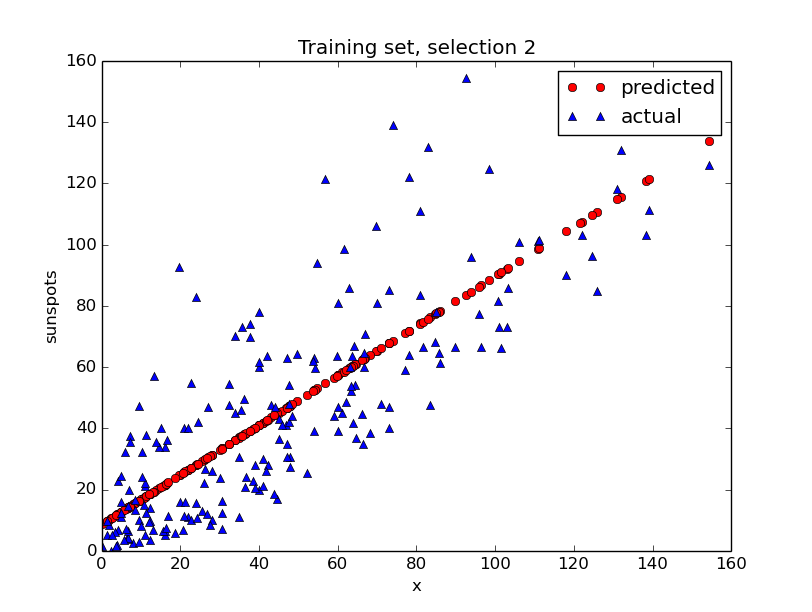
\includegraphics[width=.47\linewidth]{figures/training_set_selection2.png}
    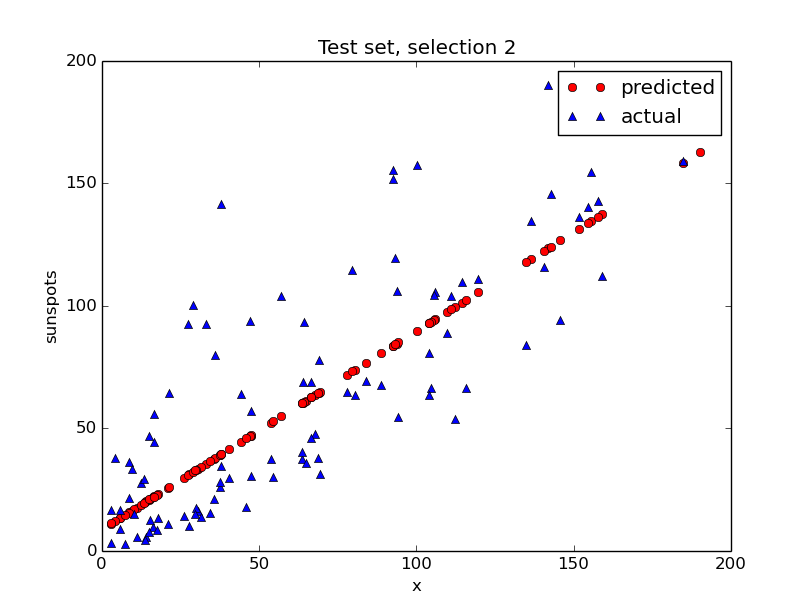
\includegraphics[width=.47\linewidth]{figures/test_set_selection2.png}
  \end{adjustwidth}
  \caption{Predicted and actual values for selection 2 of the training set and test set, plotted against the data points.}
  \label{fig:selection2}
\end{figure}

When applying the models to the test set, we get the root mean square (RMS) errors shown in figure \ref{fig:rms_ml} below.

\begin{figure}[H]
	\begin{lstlisting}
        RMS:
        Selection 1: 35.4650589931
        Selection 2: 28.8397676572
        Selection 3: 18.7700074768
	\end{lstlisting}
	\caption{Root mean square (RMS) errors when using the ML parameter estimates.}
	\label{fig:rms_ml}
\end{figure}

From the calculated RMS errors, selection 3 seems to give the best prediction, followed by selection 2 and then selection 1. Figure \ref{fig:years_vs_sunspots} shows the predicted and actual values plotted against year numbers for the years 1916-2011 of the test set. We have connected each pair of predicted and actual value by a line, so the lines ``illustrate'' what the RMS error computes. Therefore, we expect the average length of the lines to be shortest for selection 3 and longest for selection 1. Although it is hard to tell the average line length from the plots, it looks like selection 3 has quite short lines.

\begin{figure}[H]
  \begin{adjustwidth}{-7em}{-7em}
    \centering
    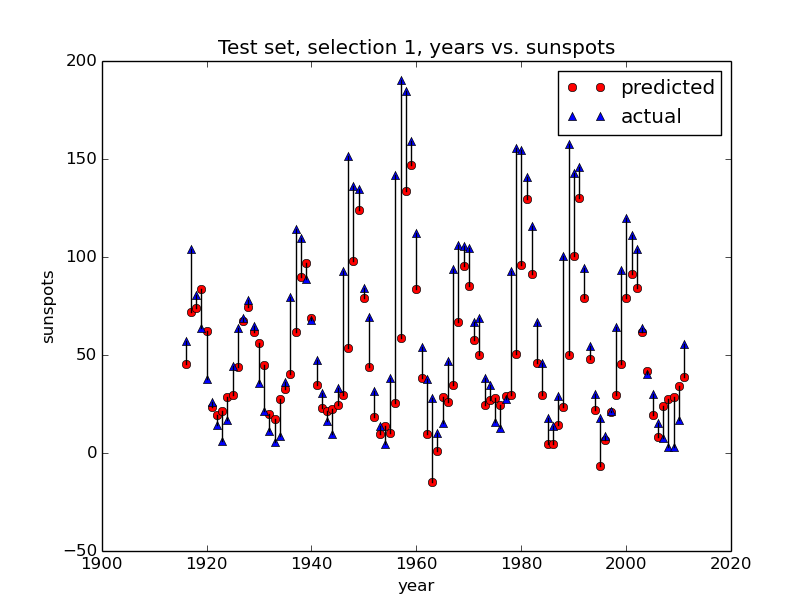
\includegraphics[width=.32\linewidth]{figures/years_vs_sunspots_selection1.png}
    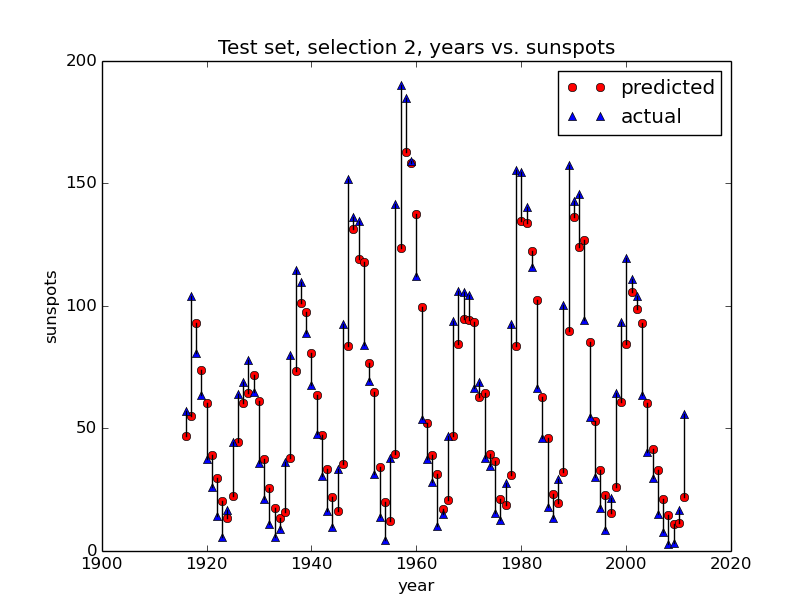
\includegraphics[width=.32\linewidth]{figures/years_vs_sunspots_selection2.png}
    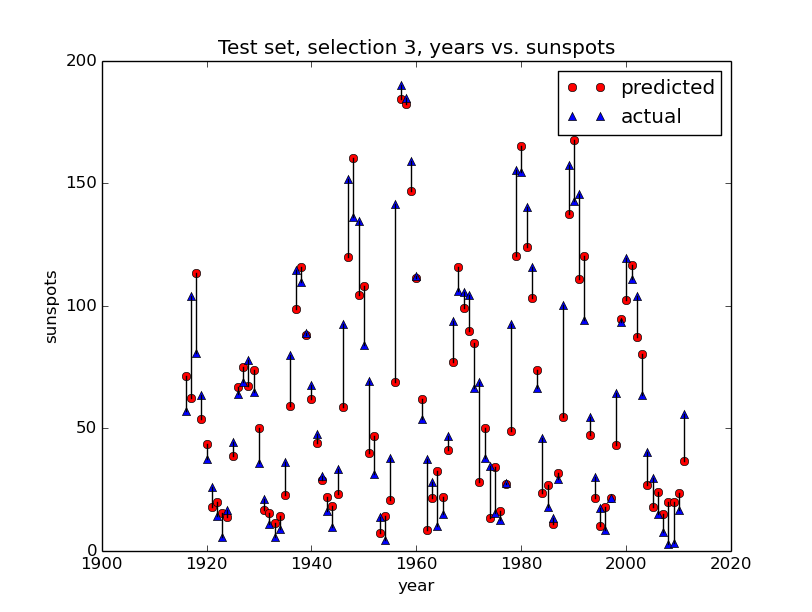
\includegraphics[width=.32\linewidth]{figures/years_vs_sunspots_selection3.png}
  \end{adjustwidth}
  \caption{Predicted and actual values plotted against year numbers, with lines connecting each predicted and actual value.}
  \label{fig:years_vs_sunspots}
\end{figure}

\subsection{Maximum a posteriori solution}
Figure \ref{fig:alpha_vs_rms_selection1} shows the RMS errors for the maximum a posteriori estimates of $w$ for selection 1, plotted against different values of $\alpha$. For comparison we have also plotted the constant RMS error for the maximum likelihood estimate of $w$. In figure \ref{fig:alpha_vs_rms_selection1a} we let $\alpha$ range from $-25$ to $11$. It looks like the MAP RMS error goes below the ML RMS error for $\alpha$ between $-18$ and $0$, so in figure \ref{fig:alpha_vs_rms_selection1b} we have zoomed in around $\alpha = -18$, and in \ref{fig:alpha_vs_rms_selection1c} we have zoomed in around 0 (note that the model is undefined for $\alpha = 0$ since we use $\alpha^{-1}$).

\begin{figure}[H]
  \begin{adjustwidth}{-7em}{-7em}
    \centering
    \begin{subfigure}{.32\linewidth}
      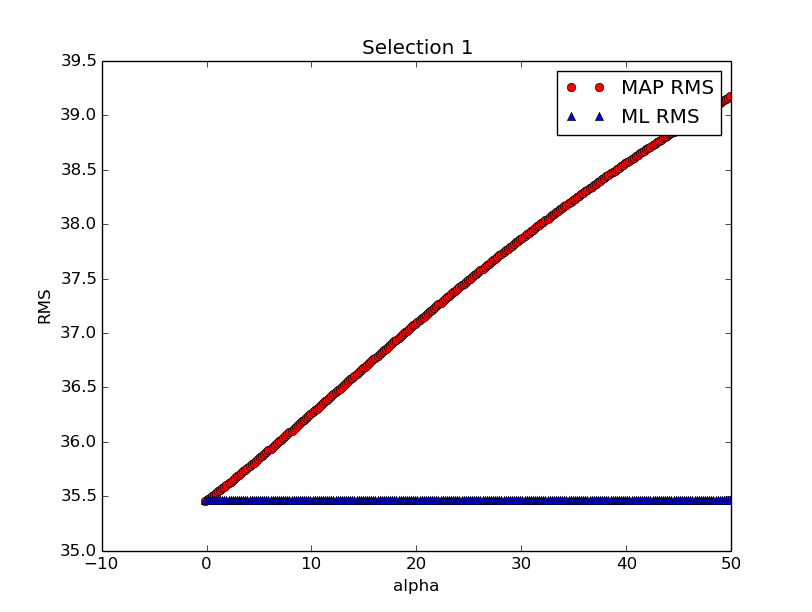
\includegraphics[width=\linewidth]{figures/alpha_vs_rms_selection1a.png}
      \caption{$\alpha$ between $-25$ and $11$.}
      \label{fig:alpha_vs_rms_selection1a}
    \end{subfigure}
    \begin{subfigure}{.32\linewidth}
      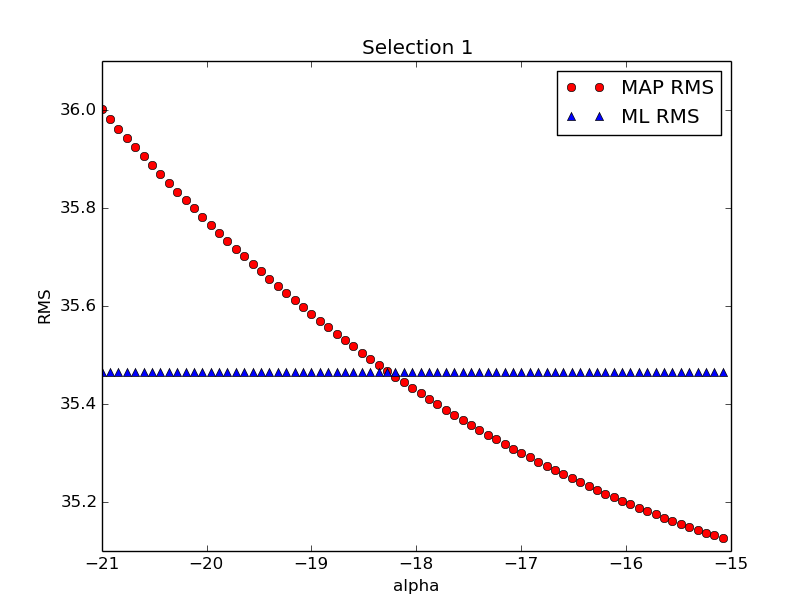
\includegraphics[width=\linewidth]{figures/alpha_vs_rms_selection1b.png}
      \caption{Zoomed in around $\alpha = -18$.}
      \label{fig:alpha_vs_rms_selection1b}
    \end{subfigure}
    \begin{subfigure}{.32\linewidth}
      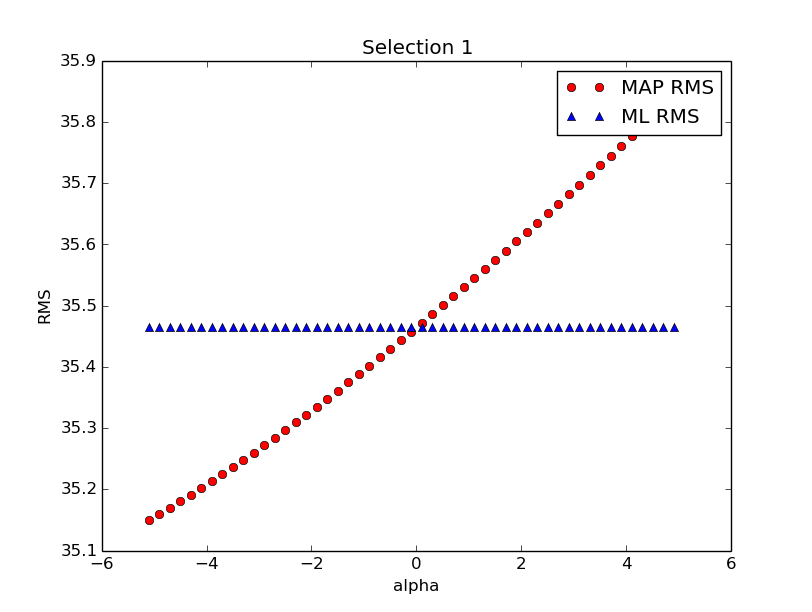
\includegraphics[width=\linewidth]{figures/alpha_vs_rms_selection1c.png}
      \caption{Zoomed in around $\alpha = 0$.}
      \label{fig:alpha_vs_rms_selection1c}
    \end{subfigure}
  \end{adjustwidth}
  \caption{RMS errors for the MAP estimate for selection 1 plotted against different values of $\alpha$ together with the constant RMS error for the ML estimate.}
  \label{fig:alpha_vs_rms_selection1}
\end{figure}

Figure \ref{fig:alpha_vs_rms_selection2} similarly shows the RMS errors for the maximum a posteriori estimates of $w$ for selection 2. Here, it looks like the MAP RMS error goes below the ML RMS error for $\alpha$ between $-15$ and $0$, so in figure \ref{fig:alpha_vs_rms_selection2b} we have zoomed in around $\alpha = -15$, and in \ref{fig:alpha_vs_rms_selection2c} we have zoomed in around 0 (still undefined for $\alpha = 0$).

\begin{figure}[H]
  \begin{adjustwidth}{-7em}{-7em}
    \centering
    \begin{subfigure}{.32\linewidth}
      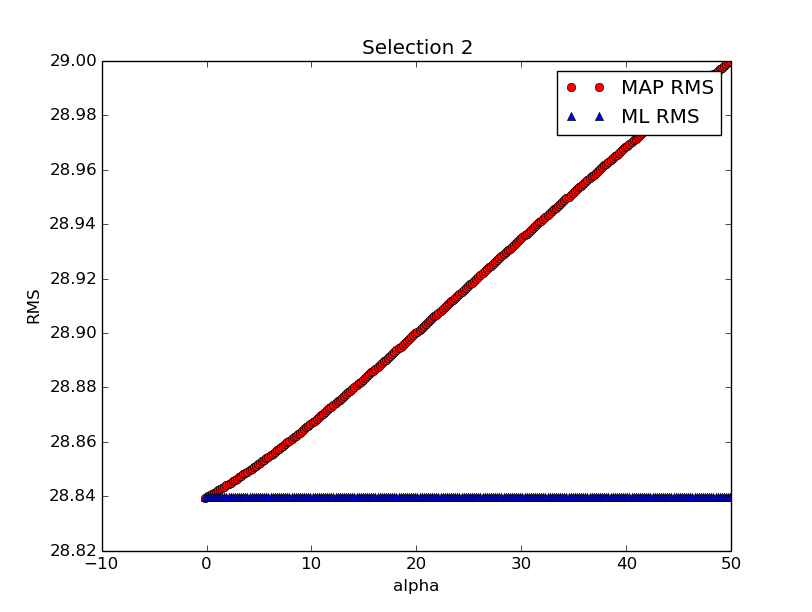
\includegraphics[width=\linewidth]{figures/alpha_vs_rms_selection2a.png}
      \caption{$\alpha$ between $-20$ and $10$.}
      \label{fig:alpha_vs_rms_selection2a}
    \end{subfigure}
    \begin{subfigure}{.32\linewidth}
      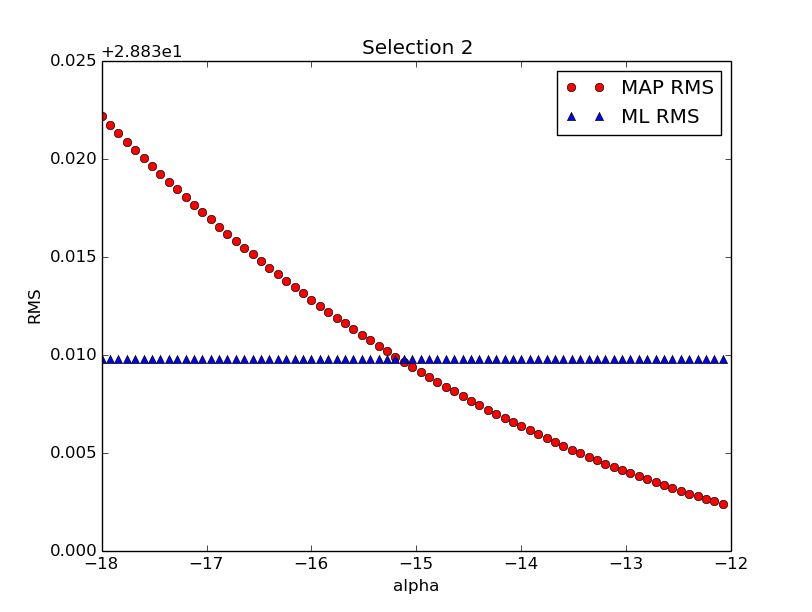
\includegraphics[width=\linewidth]{figures/alpha_vs_rms_selection2b.png}
      \caption{Zoomed in around $\alpha = -15$.}
      \label{fig:alpha_vs_rms_selection2b}
    \end{subfigure}
    \begin{subfigure}{.32\linewidth}
      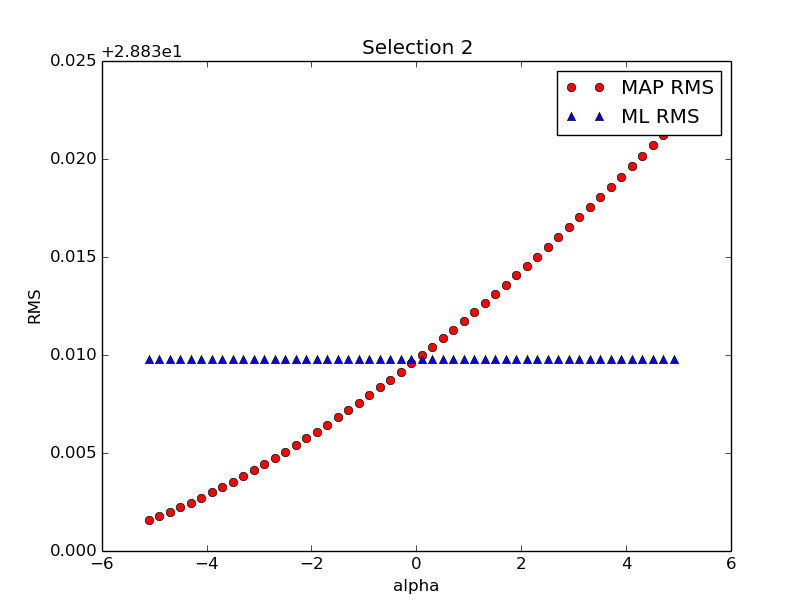
\includegraphics[width=\linewidth]{figures/alpha_vs_rms_selection2c.png}
      \caption{Zoomed in around $\alpha = 0$.}
      \label{fig:alpha_vs_rms_selection2c}
    \end{subfigure}
  \end{adjustwidth}
  \caption{RMS errors for the MAP estimate for selection 2 plotted against different values of $\alpha$ together with the constant RMS error for the ML estimate.}
  \label{fig:alpha_vs_rms_selection2}
\end{figure}

For selection 3 the RMS error seems to behave a bit differently, as figure \ref{fig:alpha_vs_rms_selection3} shows. Here, the MAP RMS error doesn't seem to go below the ML RMS error for numerically large negative values of $\alpha$. For $\alpha = -22$ the RMS error seems to skyrocket, so in figure \ref{fig:alpha_vs_rms_selection3a} we let $\alpha$ range from $-50$ to $-23$, and in figure \ref{fig:alpha_vs_rms_selection3b} we let $\alpha$ range from $-21$ to $10$. It is hard to tell from figure \ref{fig:alpha_vs_rms_selection3b} that lines actually cross, so in figure \ref{fig:alpha_vs_rms_selection3c} we have zoomed in around $\alpha = 0$.

\begin{figure}[H]
  \begin{adjustwidth}{-7em}{-7em}
    \centering
    \begin{subfigure}{.32\linewidth}
      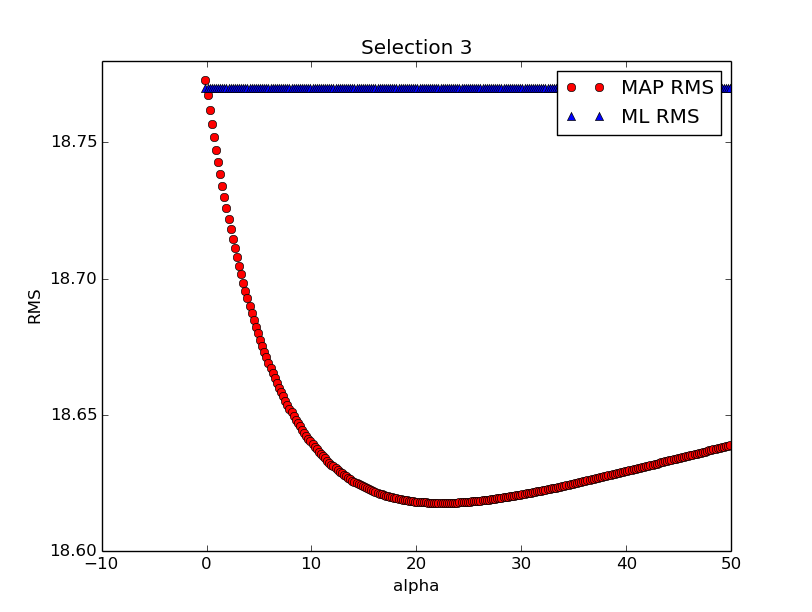
\includegraphics[width=\linewidth]{figures/alpha_vs_rms_selection3a.png}
      \caption{$\alpha$ between $-50$ and $-23$.}
      \label{fig:alpha_vs_rms_selection3a}
    \end{subfigure}
    \begin{subfigure}{.32\linewidth}
      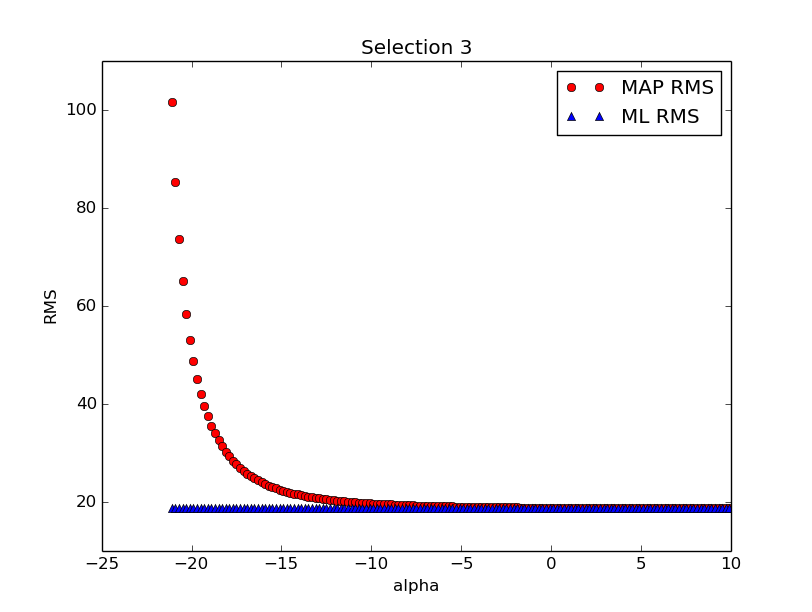
\includegraphics[width=\linewidth]{figures/alpha_vs_rms_selection3b.png}
      \caption{$\alpha$ between $-21$ and $10$.}
      \label{fig:alpha_vs_rms_selection3b}
    \end{subfigure}
    \begin{subfigure}{.32\linewidth}
      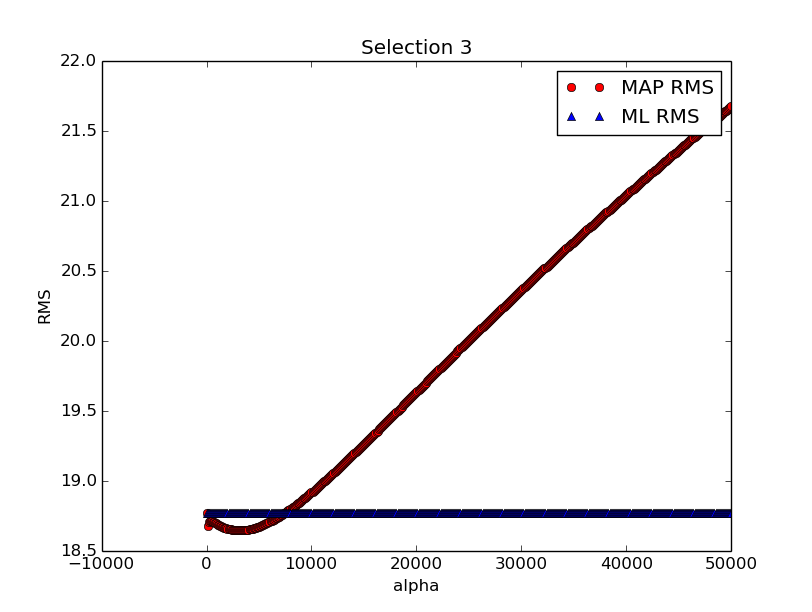
\includegraphics[width=\linewidth]{figures/alpha_vs_rms_selection3c.png}
      \caption{Zoomed in around $\alpha = 0$.}
      \label{fig:alpha_vs_rms_selection3c}
    \end{subfigure}
  \end{adjustwidth}
  \caption{RMS errors for the MAP estimate for selection 3 plotted against different values of $\alpha$ together with the constant RMS error for the ML estimate.}
  \label{fig:alpha_vs_rms_selection3}
\end{figure}

\subsection{Weighted sum-of-squares}
Given the new error function, we note that it resembles very much our previous sum-of-squares error function, defined in (3.12) in the book --- we have only added the factor $r_n$ to the expression inside the sum. Thus, we can follow the method used in formulas (3.13) to (3.15) quite closely, only modifying the formulas a little bit. When taking the gradient of the log likelihood function, we get

\begin{align*} %\label{eq:gradient}
\nabla \operatorname{ln} \, p(\bm{t} | w, \beta) = \beta \sum_{n=1}^{N} r_n \{ t_n - w^T \phi(x_n) \} \phi(x_n)^T
\end{align*}

Setting the gradient to zero gives

\begin{align*} %\label{eq:gradient_zero}
0 = \sum_{n=1}^{N} r_n t_n \phi(x_n)^T - w^T \left( \sum_{n=1}^{N} r_n \phi(x_n) \phi(x_n)^T \right)
\end{align*}

and rearranging the terms gives

\begin{align*} %\label{eq:rearranged}
w^T \left( \sum_{n=1}^{N} r_n \phi(x_n) \phi(x_n)^T \right) = \sum_{n=1}^{N} r_n t_n \phi(x_n)^T
\end{align*}

By fiddling with the sums and the corresponding matrices we see that this can be written as

\begin{align*} %\label{eq:matrices}
w^T \left( \Phi^T \mathrm{R} \Phi \right) = \bm{t}^T \mathrm{R} \Phi
\end{align*}

where we have defined $R$ to be the diagonal matrix with the weights $r_1, \dots, r_n$ on the diagonal:

\begin{align*} %\label{eq:R}
\setlength\unitlength{13pt}
R =
\left(\begin{picture}(6,3)(0,-3)
\put(1,-1){\makebox(0,0){$r_1$}}
\put(2,-2){\makebox(0,0){$r_2$}}
\put(2.8,-2.8){\makebox(0,0){$\cdot$}}
\put(3.1,-3.1){\makebox(0,0){$\cdot$}}
\put(3.4,-3.4){\makebox(0,0){$\cdot$}}
\put(5,-5){\makebox(0,0){$r_n$}}
\end{picture}
\right)
\end{align*}

Isolating $w^T$, we obtain

\begin{align*} %\label{eq:isolating}
w^T = \bm{t}^T \mathrm{R} \Phi \left( \Phi^T \mathrm{R} \Phi \right)^{-1}
\end{align*}

By transposing, we get the following expression for the solution $w^*$ that minimizes the error function:

\begin{align*} %\label{eq:transposing}
w^* &= \left( \bm{t}^T \mathrm{R} \Phi \left( \Phi^T \mathrm{R} \Phi \right)^{-1} \right) ^T
\\ &= \left( \left( \Phi^T \mathrm{R} \Phi \right)^{-1} \right)^T \Phi^T \mathrm{R} \bm{t}
\\ &= \left( \left( \Phi^T \mathrm{R} \Phi \right)^T \right)^{-1} \Phi^T \mathrm{R} \bm{t}
\\ &= \left( \Phi^T \mathrm{R} \Phi \right)^{-1} \Phi^T \mathrm{R} \bm{t}
\end{align*}

where we have used the fact that $\mathrm{R}^T = \mathrm{R}$.\\

\subsubsection{Alternative interpretations}
The weighted sum-of-squares error function is highly usable when interpreting data sets with varying degrees of noise variance or data sets with replicated data points.\\

By using weighting, data points in data sets with high noise variance can be associated with a weighing factor based on their distance from the mean, such that the closest data points have highest weighing factor, thus resulting in noisy data points counting less in the calculated error.\\

Similarly, lower weighing factors can be assigned to replicated data points in a data set to reduce the impact of these duplicated data points in the error calculation.

\end{document}
